%%%%%%%%%%%%%%%%%%%%%%%%%%%%%%%%%%%%%%%%%%%%%%%%%%%%%%%%%%%%%%%%%%%%%%%%%%%%%%%%%%%%
% Do not alter this block (unless you're familiar with LaTeX
\documentclass{article}
\usepackage[margin=1in]{geometry} 
\usepackage{amsmath,amsthm,amssymb,amssymb,amsfonts, fancyhdr, color, comment, graphicx, environ}
\usepackage{mathrsfs}

\usepackage{xcolor}
\usepackage{mdframed}
\usepackage[shortlabels]{enumitem}
\usepackage{indentfirst}
\usepackage{hyperref}
\hypersetup{
    colorlinks=true,
    linkcolor=blue,
    filecolor=magenta,      
    urlcolor=blue,
}


\pagestyle{fancy}
\usepackage{float}
\newcommand{\aboverightarrow}[1]{\xrightarrow[]{#1}}

\newenvironment{problem}[2][Problem]
    { \begin{mdframed}[backgroundcolor=gray!20] \textbf{#1 #2} \\}
    {  \end{mdframed}}

% Define solution environment
\newenvironment{solution}
    {\textit{Solution:}}
    {}
    \newcommand{\indep}{\perp \!\!\! \perp}
    \renewcommand\qedsymbol{$\blacksquare$}
\newcommand{\norm}[1]{\left\lVert#1\right\rVert}
\newcommand{\seminorm}[1]{\left [#1\right]}
\newcommand{\ts}{\textsuperscript}
\usepackage{scalerel}[2014/03/10]
\usepackage[usestackEOL]{stackengine}
\def\avint{\,\ThisStyle{\ensurestackMath{%
  \stackinset{c}{.2\LMpt}{c}{.5\LMpt}{\SavedStyle-}{\SavedStyle\phantom{\int}}}%
  \setbox0=\hbox{$\SavedStyle\int\,$}\kern-\wd0}\int}
\def\ddashint{\,\ThisStyle{\ensurestackMath{%
  \stackinset{c}{.2\LMpt}{c}{.5\LMpt+.2\LMex}{\SavedStyle-}{%
    \stackinset{c}{.2\LMpt}{c}{.5\LMpt-.2\LMex}{\SavedStyle-}{%
      \SavedStyle\phantom{\int}}}}\setbox0=\hbox{$\SavedStyle\int\,$}\kern-\wd0}\int}

\newcommand{\skipline}{$ \ $}

\newcommand{\reals}{\mathbb R}
\newcommand{\ints}{\mathbb Z}
\newcommand{\normal}{\trianglelefteq}
\newcommand{\onormal}{\trianglerighteq}

\newcommand{\subgroup}{\leqslant}

\newcommand{\sigalg}{\mathscr A}
\newcommand{\setsequence}{ \{ E_n \}_{n=1}^{\infty} }
\newcommand{\unionsetsequence}{ \bigcup_{i=1}^{\infty}  A_i }
\newcommand{\intersectionsetsequence}{ \bigcap_{i=1}^{\infty}  A_i }
\newcommand{\measureablespace}{(X, \sigalg)}
\newcommand{\measurespace}{(X, \sigalg, \mu)}
\newcommand{\borelspace}{\mathscr{B}(X)}
\newcommand{\lebesguemeasurespace}{(X, \borelspace, \lambda)}
\newcommand{\schwartzspace}{\mathcal S(\mathbb R^n)}
\newcommand{\temperedspace}{\mathcal S'(\mathbb R^n)}

\newcommand{\measure}{\mu: \sigalg \rightarrow [0, + \infty]} 
\newcommand{\outermeasure}{\mu: \mathbb{P}(X) \rightarrow [0, + \infty]} 
\newcommand{\convergesinmeasure}{\xrightarrow[\mu]{}} 
\newcommand{\convergesinLp}{\xrightarrow[L^p]{}} 

\newcommand{\convergesinschwartz}{\xrightarrow[]{\mathcal S}} 

\renewcommand{\qed}{\quad\qedsymbol}
\setlength\parindent{0pt}

% prevent line break in inline mode
\binoppenalty=\maxdimen
\relpenalty=\maxdimen

%%%%%%%%%%%%%%%%%%%%%%%%%%%%%%%%%%%%%%%%%%%%%
%Fill in the appropriate information below
\lhead{Greg DePaul}
\rhead{Stats 206} 
\chead{\textbf{Homework 5  Due: 3 November 2022}}
%%%%%%%%%%%%%%%%%%%%%%%%%%%%%%%%%%%%%%%%%%%%%

\begin{document}

\begin{problem}{1}
Under the multiple regression model (with $X$ variables $X_1, \ldots , X_{p - 1})$, show the following.
\begin{enumerate}[(a)]
\item The LS estimator of the regression intercept is:
$\hat \beta_0 = \overline Y  - \hat \beta_1 \overline X_1 - \ldots - \hat \beta_{p -1} \overline{X_{p - 1}}$,
where $\hat \beta_k$ is the LS estimator of $\beta_k$, and $\overline{X_k} = \sum_{i=1}^n X_{ik} \ (k=1, \ldots ,p - 1)$.
\emph{(Hint: Plug in $\hat \beta_1, \ldots , \hat \beta_{p - 1}$ to the least squares criterion function $Q( \cdot )$ and solve for $b_0$ that minimizes that function.)}
\item $SSE$ and the coefficient of multiple determination $R^2$ remain the same if we first center all the variables and then fit the regression model.
\emph{(Hint: Use part (a) and the fact that $SSE$ is the minimal value achieved by the least squares criterion function.)}
\end{enumerate}
\end{problem}
\begin{solution}
\begin{enumerate}[(a)]
\item Consider the criterion function 
$$Q(\hat \beta) = \sum_{i = 1}^n (Y_i - \hat \beta_0 - \hat \beta_1 X_{i1} - \ldots - \hat \beta_{p -1 } X_{i, p-1})^2$$
Differentiating with respect to $\hat \beta_0$: 
\begin{align*} 
0 = \frac{\partial Q(\hat \beta)}{\partial \hat \beta_0} &= \sum_{i = 1}^n -2 (Y_i - \hat \beta_0 - \hat \beta_1 X_{i1} - \ldots - \hat \beta_{p -1 } X_{i, p-1}) 
\end{align*}
$$0 = \sum_{i = 1}^n Y_i - \hat \beta_0 - \hat \beta_1 X_{i1} - \ldots - \hat \beta_{p -1 } X_{i, p-1}$$
$$0 = \sum_{i = 1}^n Y_i - n \hat \beta_0 - \hat \beta_1 \sum_{i = 1}^n X_{i1} - \ldots -  \hat \beta_{p -1 }  \sum_{i = 1}^n X_{i, p-1}$$
$$n \hat \beta_0 =  \sum_{i = 1}^n Y_i - \hat \beta_1 \sum_{i = 1}^n X_{i1} - \ldots -  \hat \beta_{p -1 }  \sum_{i = 1}^n X_{i, p-1}$$
$$\hat \beta_0 =  \overline{Y} - \hat \beta_1 \overline{X_{1}} - \ldots -  \hat \beta_{p -1 }  \overline{X_{p-1}}$$
\item Observe, if we centered all the variables, we get: 
\begin{align*}
SSE_{centered} &= Q_{centered}(\hat \beta) \\
&= \sum_{i = 1}^n ( (Y_i - \overline{Y}) - \hat \beta_1 (X_{i1} - \overline{X_1}) - \ldots - \hat \beta_{p -1 } (X_{i, p-1} - \overline{X_{p - 1})})^2 \\
&= \sum_{i = 1}^n (Y_i - (  \overline{Y} - \hat \beta_1 \overline{X_{1}} - \ldots -  \hat \beta_{p -1 }  \overline{X_{p-1}})- \hat \beta_1 X_{i1} - \ldots - \hat \beta_{p -1 } X_{i, p-1})^2 \\
&= \sum_{i = 1}^n (Y_i - \hat \beta_0 - \hat \beta_1 X_{i1} - \ldots - \hat \beta_{p -1 } X_{i, p-1})^2 \\
&= Q(\hat \beta) = SSE_{uncentered}
\end{align*}
Also, since $SSTO $ remains the same, we see that
$$R^2 = 1 - \frac{SSE_{centered}}{SSTO} =  1 - \frac{SSE_{uncentered}}{SSTO}$$
\end{enumerate}
\end{solution}

\begin{problem}{2}
Multiple regression: read R output. The following data set has 30 cases, one response
variable $Y$ and two predictor variables $X_1, X_2$.

\begin{table}[H]
\centering
\begin{tabular}{llll}
case & $Y$     & $X_1$    & $X_2$    \\
1    & 2.86  & 0.36  & 2.14  \\
2    & -0.50 & 0.66  & 0.74  \\
3    & 3.24  & 0.66  & 1.91  \\
4    & 0.44  & -0.52 & -0.41 \\
5    & 0.04  & -0.68 & 0.45  \\
...  & ...   & ...   & ...   \\
29   & 2.60  & 0.84  & -0.49 \\
30   & 0.98  & -0.11 & 2.41 
\end{tabular}
\end{table}
Consider fitting the nonadditive model with interaction between X1 and X2 and the R output is given below.

\begin{center}
  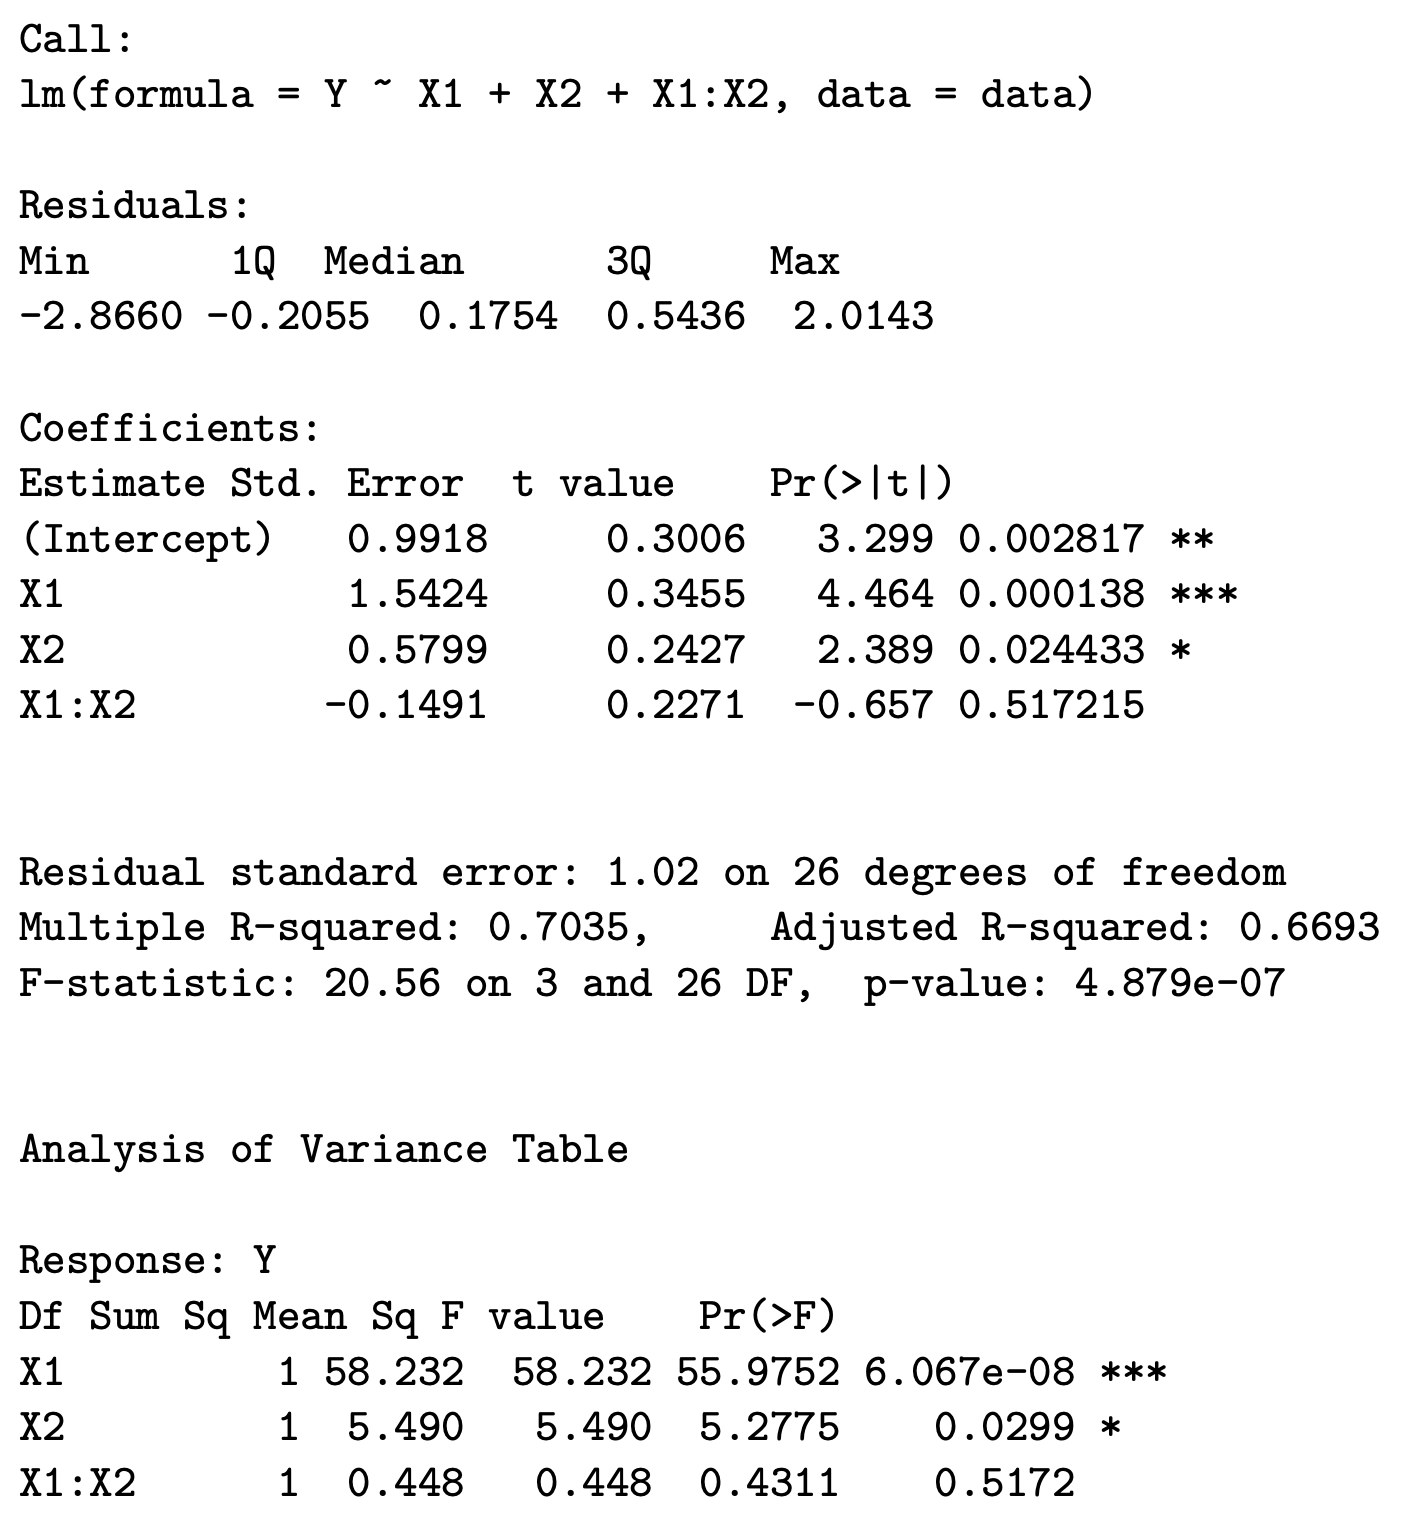
\includegraphics[width=4in]{r_output.png}
\end{center}

\begin{verbatim}
Residuals 26 27.048 1.040
\end{verbatim}

\begin{enumerate}[(a)]
\item Write down the first 4 rows of the design matrix $X$.
\item What are the regression sum of squares and error sum of squares of this model?
What is SSTO?
\item Derive the following sum of squares:
$$SSR(X1), SSE(X1), SSR(X2 | X1), SSR(X2, X1 \cdot X2 | X1)$$
$$SSR(X1 \cdot X2 | X1, X2), SSR(X1, X2), SSE(X1, X2).$$
\item We want to conduct prediction at $X_1 = 0, X_2 = 0$ and it is given that
$$(X'X)^{-1}  = \begin{pmatrix}
0.087 & -0.014 &-0.035 & -0.004 \\
-0.014 & 0.115 & -0.012 & -0.052 \\
-0.035 & -0.012 & 0.057 & -0.014 \\
- 0.004 & -0.052 & -0.014 & 0.050
\end{pmatrix}$$
What is the predicted value? What is the prediction standard error? Construct a
95\% prediction interval.
\item Test whether both $X_2$ and the interaction term $X_1X_2$ can be dropped out of the model at level 0.01. Write down the full model and the reduced model. State the null and alternative hypotheses, test statistic and its null distribution, decision rule and the conclusion.
\end{enumerate}

\end{problem}
\begin{solution}
\begin{enumerate}[(a)]
\item The first four rows of the design matrix are: 

$$X = \begin{pmatrix}
1 & 0.36 & 2.14 & 0.7704 \\
1 & 0.66 & 0.74 & 0.4884 \\
1 & 0.66 & 1.91 & 1.2606\\
1 & -0.52 & -0.41 & 0.2132 \\
\vdots & \vdots & \vdots & \vdots 
\end{pmatrix}$$
\item We see that 
$$SSR = 58.231 + 5.490 + 0.448 = 64.169$$
$$SSE = 27.048$$
$$\implies SSTO = SSR + SSE = 91.217$$
\item 
\begin{itemize}
\item $SSR(X_1) = 58.232$
\item $SSE(X_1) = SSE(X_1, X_2, X_1 \cdot X_2) + SSR(X_2, X_1 \cdot X_2 | X_1) = 27.048 + 5.938 = 32.986$
\item  $SSR(X_2 | X_1) = 5.490$
\item $SSR(X_2, X_1 \cdot X_2 | X_1) = SSR(X_1, X_2, X_1 \cdot X_2) - SSR(X_1) = 5.938$
\item $SSR(X_1 \cdot X_2 | X_1, X_2) = SSR(X_1, X_2, X_1 \cdot X_2) - SSR(X_1) - SSR(X_2 | X_1) = 0.448$
\item $SSR(X_1, X_2) = SSR(X_1) + SSR(X_2 | X_1) = 63.772$
\item $SSE(X_1, X_2) = SSE(X_1) - SSR(X_2 | X_1) = 32.986 - 5.490 = 27.496$
\end{itemize}
\item The predicted value is: 
$$\hat Y_{h}(X_1 = 0, X_2 = 0) = 0.9918$$
where 
$$X_h = \begin{pmatrix}
1 \\
0 \\
0 \\
0
\end{pmatrix}$$
We calculate the standard error of the prediction to be: 
\begin{align*}
s(pred_h) &= \sqrt{MSE \left [ 1 + X_h' (X'X)^{-1} X_h\right ]} \\
&= \sqrt{MSE \left [ 1 + \begin{pmatrix} 
1 & 0 & 0 & 0
\end{pmatrix} \begin{pmatrix}
0.087 & -0.014 &-0.035 & -0.004 \\
-0.014 & 0.115 & -0.012 & -0.052 \\
-0.035 & -0.012 & 0.057 & -0.014 \\
- 0.004 & -0.052 & -0.014 & 0.050
\end{pmatrix} \begin{pmatrix}
1 \\
0 \\
0 \\
0
\end{pmatrix}\right ]}  \\
&= \sqrt{MSE [ 1 +
0.087  ]} \\
&= \sqrt{1.040 (1 + 0.087)} \\
&= 1.0632
\end{align*}
\item We want to test the hypothesis: 

$$H_0 : \beta_2 = \beta_3 = 0 \ \ \ \text{ against } \ \ \ H_a : \beta_2 \not = 0 \text{ or } \beta_3 \not = 0$$
we choose the test statistic: 
$$F^* = \frac{\frac{SSE_{reduced} - SSE_{full}}{df_{reduced} - df_{full}}}{ \frac{SSE_{full}}{df_{full}} } = \frac{\frac{SSE(X_1) - SSE(X_1, X_2, X_3)}{2}}{ \frac{SSE(X_1, X_2, X_3)}{30 - 4}} = \frac{\frac{(32.986 - 27.048)}{2}}{\frac{27.048}{26}} = \frac{2.969}{1.040} = 2.8539$$
The null distribution is: 
$$F_{df_{reduced} - df_{full}, df_{full}} = F_{2, 26}$$
We reject provided that 
$$F^* > F_{2, 26}(1 - 0.01) = 5.526335$$
In this case, we do not have enough evidence to reject the null hypothesis. 
\end{enumerate}
\end{solution}


\begin{problem}{3}
Consider a general linear model:
$$Y_i = \beta_0 + \beta_1 X_{i1}+ \beta_2 X_{i2}+ \beta_3 X_{i3} + \epsilon_i,  \ \ \ i=1,\ldots,n.$$
Describe how you would test:
$$H_0 : \beta_1 = \beta_{1_0}, \beta_2 = \beta_{2_0} \ \ \ \text{ vs. } \ \ \ H_a : \text{not every equality in } H_0 \text{ holds},$$
where $\beta_{1_0}$ and $\beta_{2_0}$ are two prespecified constants.
\end{problem}
\begin{solution}
We define the reduced model to be: 

$$Y_{i, reduced} = \beta_0 + \beta_{1_0} X_{i1}+ \beta_{2_0} X_{i2} +\beta_3 X_{i3} + \epsilon_i $$
We would then be able to calculate the values of SSE for both the original and reduced models. 

$$SSE_{reduced} = SSE(X_3)$$
$$SSE_{full} = SSE(X_1, X_2, X_3)$$
We define the test statistic to be: 
$$F^* = \frac{\frac{SSE_{reduced} - SSE_{full}}{df_{reduced} - df_{full}}}{ \frac{SSE_{full}}{df_{full}} } \sim F_{df_{reduced} - df_{full}, df_{full}}$$
which in this case, 
$$F^* = \frac{\frac{SSE(X_3) - SSE(X_1, X_2, X_3)}{2}}{ \frac{SSE(X_1, X_2, X_3)}{n - 4}}$$
and we would reject $H_0$ provided for a given significance level $\alpha:$
$$F^* > F_{2, n - 4}(1 - \alpha)$$
\end{solution}
\end{document}